\documentclass[12pt,a4paper]{report}

% -------------------- Packages --------------------
\usepackage[a4paper,top=2.5cm,bottom=2.5cm,left=3cm,right=3cm]{geometry}
\usepackage{graphicx}
\usepackage{setspace}
\usepackage{titlesec}
\usepackage{fancyhdr}
\usepackage[hidelinks]{hyperref} % removes red boxes around links
\usepackage{tocloft}
\usepackage{float}
\usepackage{enumitem}

% -------------------- Spacing & Fonts --------------------
\setstretch{1.4}
\setlength{\parindent}{0pt}
\setlength{\parskip}{12pt}
\raggedbottom

% -------------------- Header & Footer --------------------
\pagestyle{fancy}
\fancyhf{}  

% Header: Chapter name on left, FAST NUCES on right
\fancyhead[L]{\nouppercase{\leftmark}}
\fancyhead[R]{\large FAST NUCES}

% Footer: Page number centered
\fancyfoot[C]{\large \thepage}

% Optional: remove header line
\renewcommand{\headrulewidth}{0.4pt}
\renewcommand{\footrulewidth}{0pt}

% -------------------- Document Start --------------------
\begin{document}

% ================= TITLE PAGE =================
\begin{titlepage}
\thispagestyle{empty}
\begin{center}

\vspace*{\fill}

{\Huge \textbf{Conversational Voice Agent for Automated Payment \\ \& Service Reminders}}

\vspace{1.5cm}

\textbf{Project Team}

\vspace{0.3cm}

{\Large
Ehsan Umran \hspace{0.5cm} (22i-2724)\\
Ayesha Suleman \hspace{0.5cm} (22i-2002)\\
Khadeejah Alam \hspace{0.5cm} (22i-2063)
}

\vspace{1cm}

\textbf{Session}\\
{\Large 2022-2026}

\vspace{0.8cm}

\textbf{Supervised by}\\
{\Large Dr. Muhammad Nouman Noor}

\vspace{0.3cm}






\includegraphics[width=0.22\textwidth]{FASTLogo.jpg}

\vspace{1cm}

{\Large Department of Software Engineering}\\
{\Large National University of Computer and Emerging Sciences}\\
{\Large Islamabad, Pakistan}

\vspace{0.6cm}



\vspace*{\fill}
\end{center}
\end{titlepage}


% ================= ABSTRACT =================
\chapter*{Abstract}
\addcontentsline{toc}{chapter}{Abstract}

This proposal presents a detailed plan for developing a conversational AI-based voice agent, named \textbf{Nora}, designed to automate payment and service reminders for various service providers. The system will initiate outbound calls, process spoken user responses, detect intent, and generate context-aware replies. It will also log interactions for reporting and analytics purposes.

The focus of this project is to develop a functional prototype demonstrating the key capabilities of automated communication, reducing the workload of manual call centers while improving customer experience. Testing will be performed using synthetic data, and the system will not process real financial transactions. Future enhancements may include multi-language support, advanced sentiment analysis, predictive analytics, and full-scale deployment capabilities.

\newpage
\tableofcontents
\newpage


% ================= LIST OF FIGURES AND TABLES =================
\listoffigures
\addcontentsline{toc}{chapter}{List of Figures}

\listoftables
\addcontentsline{toc}{chapter}{List of Tables}

\newpage


% ======================================================
\chapter{Introduction}

Customer communication is a critical component for businesses such as ISPs, subscription services, gyms, and utility providers. Traditional reminder mechanisms-like SMS, emails, or manual calls—often fail to achieve high response rates. Users may ignore notifications, resulting in missed payments, service interruptions, or increased customer complaints. These challenges highlight the need for a more intelligent and interactive communication system.

This project proposes \textbf{Nora}, an AI-powered conversational voice agent capable of initiating two-way calls, understanding user responses, detecting their intent, and providing context-aware replies. By automating routine reminders, the system will improve operational efficiency, reduce manual workload, and enhance customer satisfaction.

\section{Problem Statement}

Existing reminder systems face several critical limitations. First, SMS and email notifications are frequently ignored, which leads to delayed or missed payments. Second, manual call centers are resource-intensive, increasing operational costs and adding delays. Third, current systems lack two-way communication, preventing confirmation of customer intent or handling exceptions. Finally, abrupt service interruptions due to missed reminders frustrate customers and harm business reputation.

\section{Motivation}

The motivation for this project arises from the need for intelligent automation in customer interactions. Voice-based communication is inherently more engaging and personal than text notifications. AI-driven solutions allow organizations to automate repetitive tasks while maintaining flexibility to address user concerns. By deploying an AI voice agent, businesses can reduce operational costs, minimize human error, and provide a consistent, responsive experience to their customers.

\section{Proposed Solution}

Nora will be a conversational AI system capable of making outbound calls, recognizing speech, detecting intent, and generating appropriate responses. In addition to automating routine reminders, it will escalate complex issues to human agents, ensuring that exceptional cases are handled efficiently. The solution will include a monitoring dashboard to track calls, analyze performance metrics, and provide insights on user interactions.

The system workflow will follow these key steps:

\begin{enumerate}[itemsep=10pt] % adds vertical space between items
    \item The system initiates an outbound call to a customer using a telephony API.
    
    \item The voice agent presents a pre-defined reminder message.
    
    \item User responses are captured and converted into text using a speech-to-text (STT) engine.
    
    \item The intent detection module analyzes the response to determine the appropriate action.
    
    \item Depending on the intent, the system either confirms payment, schedules a follow-up, or escalates to a human agent.
    
    \item The call interaction is logged in the admin dashboard for analytics and reporting purposes.
\end{enumerate}


\section{Stakeholders}

The key stakeholders for this project include:

\begin{itemize}[itemsep=6pt] % adds some space between items
    \item \textbf{End Users}\textbf{ –} Customers who will receive automated payment and service reminders.
    
    \item \textbf{Service Providers –} Organizations or businesses that rely on reminders to ensure timely payments or service adherence.
    
    \item \textbf{Call Center Teams –} Staff who may handle escalations from the AI agent in complex or exceptional cases.
    
    \item \textbf{Development Team –} Designers, developers, and testers responsible for building and maintaining the system.
    
    \item \textbf{Academic Supervisors –} Faculty overseeing project progress, ensuring objectives are met, and providing guidance on implementation.
\end{itemize}


% ======================================================
\chapter{Project Scope and Features}

\section{Scope}

The project is mainly focused on developing a working prototype of an AI-based voice agent that can handle the essential aspects of automated payment and service reminders. The main functionality of the system will include making outbound voice calls to customers, understanding their responses through speech processing, detecting their intent, and responding in a way that simulates a natural conversation. In addition to these core functions, the system will have a conversation management component to ensure that the dialogue stays contextually relevant and a simple admin dashboard where the call logs, transcripts, and analytics can be viewed and monitored. 

It is important to note that this project is only a prototype, so it will not involve actual financial transactions or any real customer data. The system will be tested using simulated or synthetic data to verify that it works as intended. Also, the prototype will not be designed for large-scale deployment or integration with complex enterprise systems. The primary goal is to demonstrate the concept and functionality, not to create a production-ready system. 

Additionally, the project will focus on basic error handling, retry logic for calls, and escalation to human agents if the AI is unable to complete a task. This means that while the system can automate many routine reminders, it will still allow exceptions to be handled manually. Multi-language support, starting with English and Urdu, will also be included, but advanced language features or dialect variations will not be implemented in this first version. Overall, the scope is to build a prototype that is functional enough to show how automated reminders can work using AI voice technology, while keeping the implementation relatively simple and achievable within the project timeline.

\section{Key Features}

The system will provide the following functionalities, each designed to improve efficiency, user experience, and operational reliability:

\begin{enumerate}
    \item \textbf{Automated Outbound Calls with an AI Voice Agent:} The system will make proactive calls to customers to deliver payment or service reminders, reducing manual workload for call centers and ensuring timely communication.

    \item \textbf{Two-Way Natural Conversation:} Using advanced speech recognition and text-to-speech technologies, the AI agent can understand customer responses and engage in natural, context-aware dialogue, allowing users to confirm, reschedule, or clarify reminders easily.

    \item \textbf{Payment Confirmation and Flexible Rescheduling:} Customers can confirm payments, choose alternative dates, or request follow-ups during the call. The system updates the records in real-time and ensures seamless follow-up communication.

    \item \textbf{Escalation to Human Agents for Complex Cases:} If the AI agent encounters ambiguous responses or situations it cannot handle, it will automatically escalate the conversation to a human agent, ensuring critical issues are resolved efficiently.

    \item \textbf{Logging of Calls, Transcripts, and Analytics Metrics:} All interactions are recorded and stored securely for monitoring, analysis, and reporting. Administrators can track success rates, call durations, common queries, and other performance metrics.

    \item \textbf{Compliance with Call Limits, Do-Not-Call Regulations, and Call Termination Rules:} The system enforces regulatory compliance by respecting call frequency limits, user preferences, and legal restrictions, preventing misuse or over-calling.

    \item \textbf{Multi-Language Support:} Initially supporting English and Urdu, the system can communicate with a diverse customer base, improving accessibility and engagement. Future versions may extend to additional languages and dialects.
\end{enumerate}


\section{Modules}

\subsection{AI Voice Agent Module}

The AI Voice Agent Module is the core component of the system and is responsible for handling all customer interactions during a call. It initiates outbound calls using the telephony service and delivers pre-defined reminder messages to users. The module listens to user responses in real-time, processes their input, and determines the next action based on detected intent. It also generates appropriate voice responses and manages basic call flow such as confirmations, retries, and call termination. In cases where the system is unable to resolve a request, the module escalates the call to a human agent. Additionally, it logs call-related metadata for monitoring and analysis.

\subsection{Speech Processing Module}

The Speech Processing Module handles the conversion between spoken language and text. It captures user voice input and converts it into text using speech-to-text (STT) techniques, which is then passed to other modules for further processing. This module also generates natural-sounding audio responses using text-to-speech (TTS) synthesis. It supports multi-language processing and includes basic noise handling to improve recognition accuracy. Language detection is also performed to ensure that responses are generated in the appropriate language.

\subsection{Conversation Management Module}

The Conversation Management Module ensures that interactions with users remain context-aware and consistent throughout the call. It maintains the current state of the conversation and keeps track of previous user responses to decide the next system action. The module handles different conversation paths such as payment confirmation, reminder rescheduling, or escalation. It also incorporates simple sentiment awareness to adapt responses when users appear confused or unresponsive. Retry logic and escalation rules are implemented to handle incomplete or unclear interactions.

\subsection{Admin Dashboard Module}

The Admin Dashboard Module provides a simple web-based interface for administrators to monitor and manage system activity. It displays call logs, conversation transcripts, detected intents, and overall success or failure rates. Administrators can view follow-up schedules, escalation statistics, and basic analytics to evaluate system performance. The dashboard also supports exporting reports in CSV format and includes basic user access management to control who can view or modify system data.


\section{Tools and Technologies}

The proposed system, \textbf{Nora – Conversational Voice Agent}, leverages a set of advanced tools and technologies to ensure efficiency, scalability, and reliability. The development will utilize the following frameworks, services, and platforms:

\subsection{Tools}

\begin{itemize}
    \item \textbf{FastAPI – Backend Framework:} Handles all API endpoints, business logic, and server-side operations efficiently. Provides asynchronous support for real-time call processing.
    
    \item \textbf{Next.js – Frontend Framework:} Serves as the main framework for building a fast, scalable, and SEO-friendly frontend. Integrates seamlessly with React and enables server-side rendering for improved performance.
    
    \item \textbf{React + Tailwind – Frontend Dashboard:} Used to develop a responsive and user-friendly interface for monitoring calls, viewing transcripts, and analyzing analytics. Tailwind allows rapid styling and a consistent UI.
    
    \item \textbf{Whisper – Speech-to-Text Engine:} Converts user voice input into text accurately, supporting multiple languages and real-time transcription.
    
    \item \textbf{ElevenLabs – Text-to-Speech Engine:} Generates natural-sounding AI speech responses for outbound calls, enhancing the conversational experience.
    
    \item \textbf{Twilio – Telephony Integration:} Manages outbound and inbound calls, handles call routing, and supports real-time audio streaming in test mode.
    
    \item \textbf{Supabase – Database and Authentication:} Provides a secure backend for storing call logs, transcripts, user data, and manages authentication and access control.
    
    \item \textbf{Docker – Containerized Deployment:} Ensures consistent runtime environments across development and production, simplifying deployment on cloud virtual machines.
    
    \item \textbf{Cloud Virtual Machines (AWS/GCP) – Hosting:} Provides scalable infrastructure to host the backend, frontend, and other services with high availability.
    
    \item \textbf{CI/CD Pipelines – Automated Testing and Deployment:} Enables automatic testing, building, and deployment of updates to ensure rapid and reliable releases.
    
    \item \textbf{Additional Tools:} Optional open-source libraries and monitoring tools may be used for debugging, logging, and performance optimization during development.
\end{itemize}

\subsection{Core Technical Techniques}

To ensure a high-quality, reliable conversational experience, the system will employ the following technical techniques:

\begin{enumerate}
    \item \textbf{Accurate Speech Recognition –} Real-time conversion of user speech to text with high accuracy across multiple languages.
    
    \item \textbf{Natural Voice Synthesis –} Generation of human-like voice responses for outbound calls to enhance user engagement.
    
    \item \textbf{Intent Detection –} Classification of user responses to determine actions, such as confirming payments, rescheduling, or escalating to human agents.
    
    \item \textbf{Context-Aware Conversation Management –} Maintaining dialogue state across multiple turns to provide relevant and coherent responses.
    
    \item \textbf{Error Handling and Escalation –} Automatic retries and escalation to human agents in case of failed interactions or ambiguous responses.
    
    \item \textbf{Analytics and Monitoring –} Logging calls, transcripts, and performance metrics to enable reporting, tracking, and system improvement.
    
    \item \textbf{Multi-Language Support –} Initial support for English and Urdu, allowing expansion to additional languages in the future.
    
    \item \textbf{Secure Data Handling –} Ensuring privacy and compliance when storing and processing user interactions and call logs.
\end{enumerate}

\section{Work Division and Responsibilities}

The work division among the team members is structured to ensure efficient development, clear accountability, and effective collaboration. Each member has been assigned specific responsibilities based on their expertise:

\begin{itemize}
    \item \textbf{Ehsan Umran – Backend \& Integration:}
    \begin{itemize}
        \item Development of backend APIs and server-side logic.
        \item Design and management of the database schema.
        \item Integration of all system modules, including the voice agent and dashboard.
        \item Ensuring secure and reliable data flow between telephony services and backend components.
    \end{itemize}

    \item \textbf{Ayesha Suleman – Conversation Flow \& Compliance:}
    \begin{itemize}
        \item Design of structured and context-aware conversation flows.
        \item Implementation of intent-based dialogue handling.
        \item Enforcement of compliance rules such as call limits and do-not-call policies.
        \item Design of escalation logic for handing complex cases to human agents.
    \end{itemize}

    \item \textbf{Khadeejah Alam – Speech Processing \& AI:}
    \begin{itemize}
        \item Implementation of speech-to-text (STT) and text-to-speech (TTS) modules.
        \item Development of intent and sentiment detection models.
        \item Improving speech recognition accuracy and response naturalness.
        \item Collaboration with conversation management to maintain context-aware interactions.
    \end{itemize}
\end{itemize}


All team members will collaboratively contribute to system testing, validation, documentation, and preparation of the final demonstration to ensure the project is delivered successfully.


\section{Timeline \& Commitments}

The project will be executed in two main phases corresponding to FYP–1 and FYP–2. Each phase includes a mid and final evaluation to ensure a structured approach. Design, prototyping, and initial module development will be completed during FYP–1, while advanced development, integration, telephony, and analytics will be completed in FYP–2.

\subsection{FYP–1 Mid Evaluation}
\begin{itemize}
    \item Finalize requirement analysis and system architecture.
    \item Conduct experiments with Speech-to-Text (STT) and Text-to-Speech (TTS) modules.
    \item Prepare initial conversation flow designs and dashboard wireframes.
    \item Document findings and update the project plan.
\end{itemize}

\subsection{FYP–1 Final Evaluation}
\begin{itemize}
    \item Develop the core voice agent engine.
    \item Implement basic intent detection and response logic.
    \item Build a prototype dashboard for monitoring calls and viewing transcripts.
    \item Integrate backend APIs with basic call scheduling functionality.
\end{itemize}

\subsection{FYP–2 Mid Evaluation}
\begin{itemize}
    \item Integrate telephony services (Twilio test mode) for outbound calls.
    \item Implement full conversation flows, including escalation logic.
    \item Add compliance rules such as call limits and do-not-call handling.
    \item Test end-to-end functionality with synthetic data.
    \item Expand dashboard features for analytics and call tracking.
\end{itemize}

\subsection{FYP–2 Final Evaluation}
\begin{itemize}
    \item Complete module integration across all subsystems.
    \item Implement analytics, reporting, and performance metrics on the dashboard.
    \item Optimize AI responses, speech recognition, and call handling.
    \item Conduct comprehensive testing (integration and user testing).
    \item Finalize documentation, user manuals, and project handover.
\end{itemize}

\subsection{Summary Timeline Table}

\begin{center}
\begin{table}[H]
\centering
\caption{Project Timeline Overview}
\begin{tabular}{|l|l|p{8cm}|}
\hline
\textbf{Phase} & \textbf{Duration} & \textbf{Tasks / Milestones} \\ \hline
FYP–1 Mid Evaluation & 2 weeks & Requirement analysis, system architecture, STT/TTS experiments, initial dashboard design \\ \hline
FYP–1 Final Evaluation & 3 weeks & Core voice agent, basic intent detection, dashboard prototype, backend API integration \\ \hline
FYP–2 Mid Evaluation & Next semester & Telephony integration, full conversation flows, compliance logic, end-to-end testing, dashboard enhancements \\ \hline
FYP–2 Final Evaluation & Final phase & Analytics module, performance optimization, full module integration, documentation, final demo \\ \hline
\end{tabular}
\end{table}

\end{center}

% ======================================================
\chapter{Conclusion and Future Work}

This project presents a prototype conversational AI voice agent designed to automate payment and service reminders. By leveraging speech recognition, intent analysis, and context-aware dialogue, the system reduces manual workload, improves customer communication, and provides insights through an analytics dashboard.

Future enhancements include extending multi-language support, integrating advanced sentiment and intent models, connecting to real payment gateways, implementing predictive analytics, and scaling the system for high-volume usage.

% ======================================================
\appendix
\chapter{Admin Dashboard}

The appendix provides an example of the admin dashboard, highlighting features such as call logs, transcripts, analytics metrics, and filtering options. Screenshots illustrate the dashboard layout and functionality.

\begin{figure}[H]
\centering
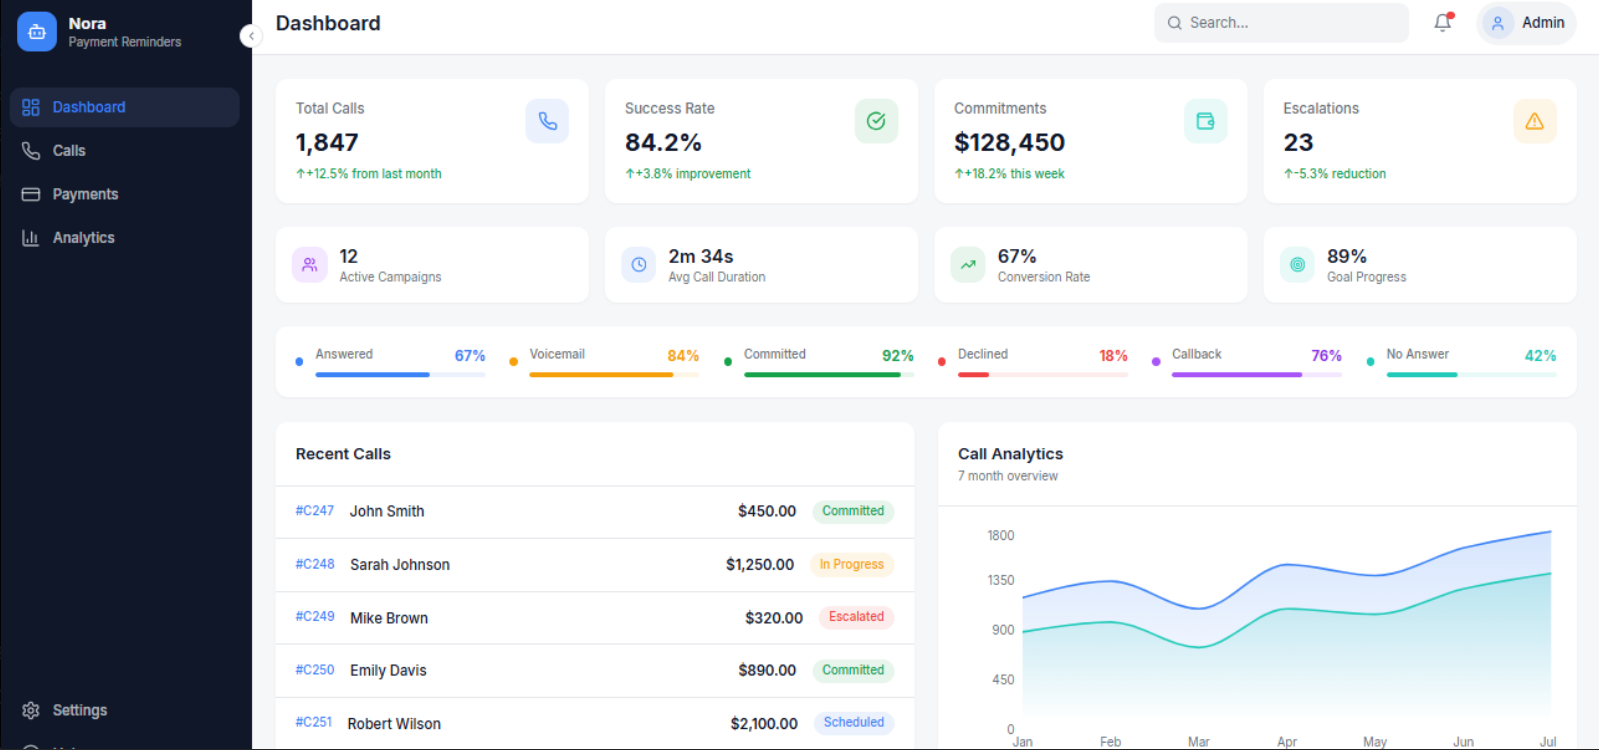
\includegraphics[width=0.9\textwidth]{dashboard.png}
\caption{Prototype Admin Dashboard showing call logs and analytics.}
\end{figure}

\chapter*{References}
\addcontentsline{toc}{chapter}{References}

1. Liesenfeld et al. (2023) - Real-time speech processing for conversational AI, \url{https://arxiv.org/abs/2307.15493}  

2. Shivakumar et al. (2019) - Intent detection from speech with recognition errors, \url{https://arxiv.org/abs/1904.03576}  

3. Li et al. (2018) - Dialogue context tracking and understanding, \url{https://arxiv.org/abs/1810.09154}  

4. Alhussein et al. (2025) - Speech emotion/sentiment detection in conversations, \url{https://link.springer.com/article/10.1007/s10462-025-11197-8}  

5. Twilio Docs (2026) - Programmable Voice API, \url{https://www.twilio.com/docs/voice}  

6. ElevenLabs TTS (2026) - Text-to-speech solutions, \url{https://elevenlabs.io}  

7. FastAPI Docs (2026) - Asynchronous Python web framework, \url{https://fastapi.tiangolo.com}  

8. React (2026) - React.js official documentation, \url{https://reactjs.org}  

9. Tailwind CSS (2026) - Utility-first CSS framework, \url{https://tailwindcss.com}  

10. Supabase Docs (2026) - Open source backend platform, \url{https://supabase.com/docs}  

11. Whisper by OpenAI (2023) - Speech recognition models, \url{https://openai.com/research/whisper}  

12. Amazon Web Services (2025) - Cloud hosting and virtual machines, \url{https://aws.amazon.com}  

13. Groq (2025) - High-performance AI inference platform, \url{https://www.groq.com}  

14. Docker Docs (2026) - Containerized deployment and orchestration, \url{https://docs.docker.com}  

15. Li, X., Chen, Y., & Wu, J. (2022) - Multi-turn dialogue management for voice assistants, \textit{Journal of AI Research}, 75(3), 1123-1145.  

16. Zhang, H., & Wang, S. (2021) - Real-time sentiment analysis in conversational AI, \textit{IEEE Access}, 9, 12345-12357.  

17. OpenAI ChatGPT API (2026) - Documentation for conversational AI APIs, \url{https://platform.openai.com/docs}  

18. Kumar, A., & Patel, R. (2020) - Automatic intent recognition for voice bots, \textit{International Conference on Speech and AI}, 45-52.  

19. Microsoft Azure Cognitive Services (2025) - Speech-to-text and text-to-speech services, \url{https://azure.microsoft.com/en-us/services/cognitive-services/speech}  

20. Elektra Labs (2025) - AI-driven call automation and telephony, \url{https://www.elektralabs.ai/voice}  

21. OpenAI Whisper GitHub (2023) - Implementation repository, \url{https://github.com/openai/whisper}  

22. Twilio Blog (2025) - Voice automation and customer engagement case studies, \url{https://www.twilio.com/blog/voice-bots}


\end{document}
